\documentclass{standalone}
\usepackage[utf8]{inputenc}
\usepackage{amsmath}
\usepackage{amsfonts}
\usepackage{amssymb}
\usepackage{tikz}
\usetikzlibrary{calc}

% GanttHeader setups some parameters for the rest of the diagram
% #1 Width of the diagram
% #2 Width of the space reserved for task numbers
% #3 Width of the space reserved for task names
% #4 Number of months in the diagram
% In addition to these parameters, the layout of the diagram is influenced
% by keys defined below, such as y, which changes the vertical scale
\def\GanttHeader#1#2#3#4{%
 \pgfmathparse{(#1-#2-#3)/(#4)}
 \tikzset{y=7mm, task number/.style={left, font=\bfseries},
     task description/.style={text width=#3,  right, draw=none,
           font=\sffamily, xshift=#2,
           minimum height=2em},
     gantt bar/.style={draw=black, fill=blue!30},
     help lines/.style={draw=black!30, dashed},
     x=\pgfmathresult pt
     }
  \def\totalmonths{#4}
  \node (Header) [task description] at (0,0) {\textbf{\large }};
  \begin{scope}[shift=($(Header.south east)$)]
    \foreach \x in {1,...,#4}
      \node[above,rotate=90] at (\x,1) {\tiny\x};
 \end{scope}
}

% This macro adds a task to the diagram
% #1 Number of the task
% #2 Task's name
% #3 Starting date of the task (month's number, can be non-integer)
% #4 Task's duration in months (can be non-integer)
\def\Task#1#2{%
%\node[task number] at ($(Header.west) + (0, -#1)$) {#1};
\node[task description] at (0,-#1) {#2};
\begin{scope}[shift=($(Header.south east)$)]
  \draw (0,-#1) rectangle +(\totalmonths, 1);
  \foreach \x in {1,...,\totalmonths}
    \draw[help lines] (\x,-#1) -- +(0,1);
\end{scope}
}

% This macro adds a task to the diagram
% #1 Number of the task
% #2 Task's name
% #3 Starting date of the task (month's number, can be non-integer)
% #4 Task's duration in months (can be non-integer)
\def\TaskActive#1#2#3{%
\begin{scope}[shift=($(Header.south east)$)]
  \filldraw[gantt bar] ($(#2, -#1+0.2)$) rectangle +(#3,0.6);
\end{scope}
}

\begin{document}

\begin{tabular}{l}
\begin{tabular}{lr}
Scheduler: & FIFO scheduler
\\
Input: & input/testdata2.txt
\\
Total Process Count: & 11
\\
Total Waiting Time: & 674
\\
Average Waiting Time: & 61.272728
\\
Total Turnaround Time: & 806
\\
Average Turnaround Time: & 73.27273
\\
Total Context Switch Count: & 11
\\
\end{tabular}
\\
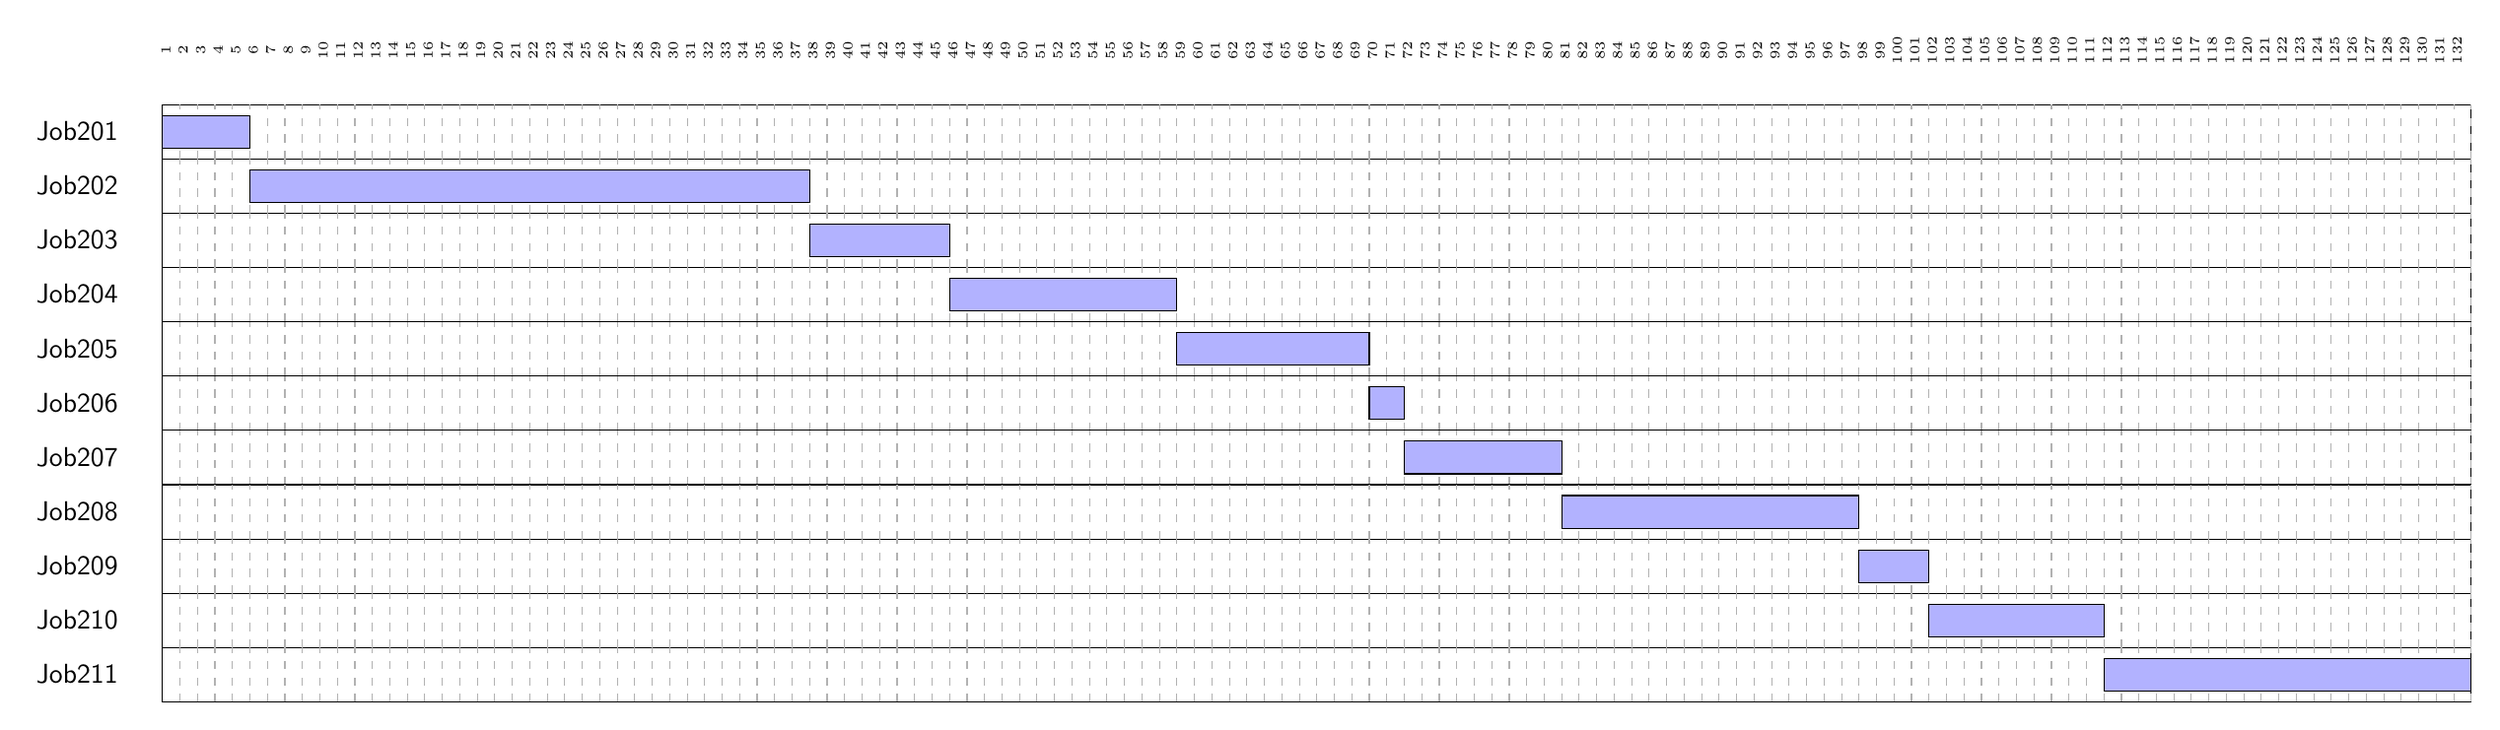
\begin{tikzpicture}
\GanttHeader{32cm}{5ex}{1.5cm}{132}
\Task{1}{Job201}
\Task{2}{Job202}
\Task{3}{Job203}
\Task{4}{Job204}
\Task{5}{Job205}
\Task{6}{Job206}
\Task{7}{Job207}
\Task{8}{Job208}
\Task{9}{Job209}
\Task{10}{Job210}
\Task{11}{Job211}
\TaskActive{1}{0}{5}
\TaskActive{2}{5}{32}
\TaskActive{3}{37}{8}
\TaskActive{4}{45}{13}
\TaskActive{5}{58}{11}
\TaskActive{6}{69}{2}
\TaskActive{7}{71}{9}
\TaskActive{8}{80}{17}
\TaskActive{9}{97}{4}
\TaskActive{10}{101}{10}
\TaskActive{11}{111}{21}
\end{tikzpicture}
\end{tabular}
\end{document}
